\documentclass[10.5pt,a4paper]{article}
\usepackage[utf8]{inputenc}
\usepackage[T1]{fontenc}
\usepackage{lmodern,microtype}
\usepackage[margin=20mm]{geometry}
\usepackage{amsmath,amssymb,booktabs,graphicx,float,caption}
\usepackage[colorlinks=true,allcolors=black]{hyperref}
\captionsetup{font=small,labelfont=bf}

\title{\vspace{-14mm}\textbf{Angular responsivity models of the photodiode (Thorlabs PDA100A2)}}
\author{Kevin Acu\~na-Condori}
\date{October 2026}

\begin{document}
\maketitle
\vspace{-6mm}

\noindent The received signal strength of the single-LED system is
\begin{equation}
  \mathrm{RSS} = A\,R(\psi)\,\cos^{m}\phi\,/\,d^{2},\qquad \cos\psi = \mathbf n^{\mathsf T}\mathbf u ,
\end{equation}
where $\psi$ is the incidence angle on the PD (normal $\mathbf n$, direction to the LED $\mathbf u$),
$\phi$ the emission angle, $d$ the distance, and $R(\psi)$ the normalized angular responsivity of the PD
($R(0)=1$). Three models of $R$ were compared; the values below are the ones currently used
(\path{demo/config/demo.toml}, implementation in \path{demo/vlp/responses.py}).

\section*{1. SQ model (Bastiaens et al., IEEE Access 2020) --- used}
\begin{equation}
  R_{\rm SQ}(\psi) = \max\!\left(0,\; 1 - a\,\psi^{2}\right),\qquad
  a = \frac{1 - 1/\sqrt{2}}{\psi_{3\rm dB}^{2}} .
\end{equation}
It is quadratic in the angle itself (not in its cosine), and $R_{\rm SQ}(\psi_{3\rm dB}) = 1/\sqrt2$. It
has a natural zero at $\psi_0 = 1/\sqrt{a}$, so no separate field of view is needed.

\section*{2. Generalized Lambertian model}
\begin{equation}
  R_{\cos^{m_R}}(\psi) = \begin{cases} \cos^{m_R}\psi, & \psi \le \psi_{\rm FOV}\\ 0, & \psi > \psi_{\rm FOV}\end{cases}
\end{equation}

\section*{3. Lambertian model}
\begin{equation}
  R_{\cos}(\psi) = \begin{cases} \cos\psi, & \psi \le \psi_{\rm FOV}\\ 0, & \psi > \psi_{\rm FOV}\end{cases}
\end{equation}

\begin{table}[H]\centering\small
\begin{tabular}{llll}\toprule
Model & Parameter & Value & Source\\\midrule
SQ & $\psi_{3\rm dB}$ & 0.61\,rad ($34.95^\circ$) & Bastiaens 2020, Table 1 (PDA100A2)\\
   & $a$ & 0.7871\,rad$^{-2}$ & from $\psi_{3\rm dB}$\\
   & zero $\psi_0 = 1/\sqrt a$ & 1.127\,rad ($64.58^\circ$) & from $\psi_{3\rm dB}$\\
$\cos^{m_R}$ & $m_R$ & 1.9 & Bastiaens 2020, Table 1 (PDA100A2)\\
 & $\psi_{\rm FOV}$ & $64^\circ$ & hard cut-off (close to the SQ zero)\\
$\cos$ & $\psi_{\rm FOV}$ & $64^\circ$ & hard cut-off\\\bottomrule
\end{tabular}
\caption{Parameters currently used.}
\end{table}

\begin{figure}[H]\centering
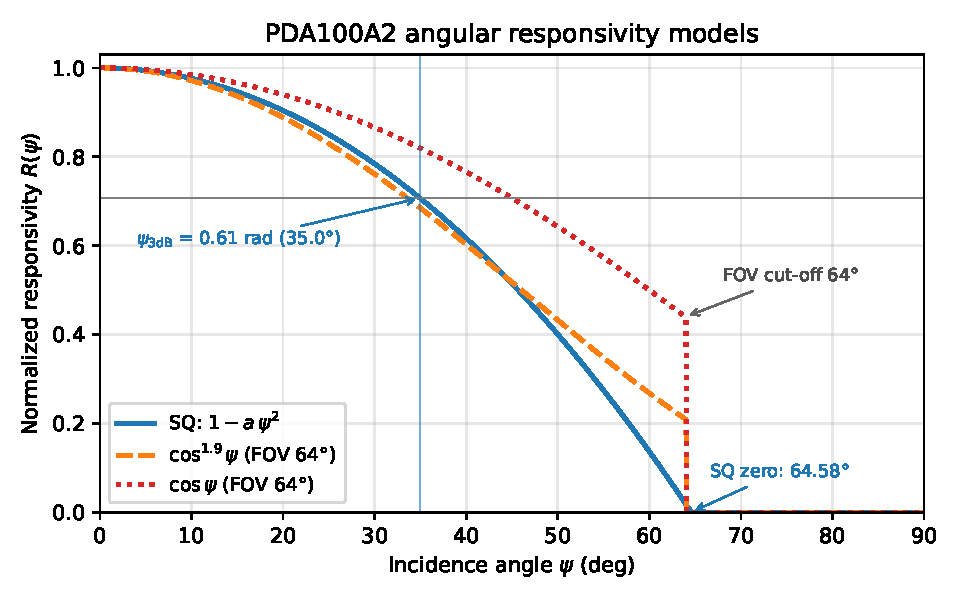
\includegraphics[width=0.78\linewidth]{pd_response.pdf}
\caption{The three models with the values of the table. The horizontal line marks $1/\sqrt2$.}
\end{figure}

\section*{Effect on 3D positioning (experiment 01)}
\noindent On the 125 positions of the two $K=10$ campaigns (NLS estimator), with $A$ and $m$ refitted for
each PD model from the same horizontal scan:

\begin{table}[H]\centering\small
\begin{tabular}{lccc}\toprule
& SQ & $\cos^{1.9}\psi$ & $\cos\psi$\\\midrule
Mean 3D error & \textbf{3.92\,cm} & 8.42\,cm & 77.4\,cm\\
Fitted Lambertian order $m$ of the LED & 6.15 & 5.89 & 6.79\\\bottomrule
\end{tabular}
\end{table}

\noindent \textbf{Shape test.} The shape of the $K$ RSS, independent of $A$ and $m$, gives an rms
deviation of 1.76\,\% for SQ, 1.91\,\% for $\cos^{1.9}$ and 7.15\,\% for $\cos$ (nominal geometry).
\textbf{Adapter tilt.} The adapter tilt inferred from those shapes is $14.8^\circ$ (SQ, corrected $Z$
scale), $14.5^\circ$ ($\cos^{1.9}$) and $24.9^\circ$ ($\cos$), against a physical value of $15^\circ$.
\textbf{Conclusion.} The Lambertian model is clearly rejected. SQ and $\cos^{1.9}$ fit the shapes
similarly, but SQ halves the 3D error. These results use the LED at $(270, 890)$\,mm.

\end{document}
